% file: thesis.tex
\documentclass[a4paper,twoside,12pt,nochapterprefix]{scrbook}


\usepackage{amsmath,amssymb,amsthm}
\usepackage[footnotesize,sl,SL,hang,tight]{subfigure}  % helpful package for aligning figures next to each other
\usepackage{longtable} % tables over several pages
\usepackage[font={small,sl},hang,labelfont=bf]{caption} % configure captions
\usepackage{booktabs} % publication quality tables for LaTeX
%\usepackage{showkeys} % shows the labels above the references for easier development
\usepackage{listings}
\usepackage{acronym}         %Abkürzungsverzeichnis
\usepackage{color} %red, green, blue, yellow, cyan, magenta, black, white
\definecolor{mygreen}{RGB}{28,172,0} % color values Red, Green, Blue
\definecolor{mylilas}{RGB}{170,55,241}
\lstset{language=Matlab,%
	frame=top,frame=bottom,
	%basicstyle=\color{red},
	breaklines=true,%
	morekeywords={matlab2tikz},
	keywordstyle=\color{blue},%
	morekeywords=[2]{1}, keywordstyle=[2]{\color{black}},
	identifierstyle=\color{black},%
	stringstyle=\color{mylilas},
	commentstyle=\color{mygreen},%
	showstringspaces=false,%without this there will be a symbol in the places where there is a space
	numbers=left,%
	numberstyle={\tiny \color{black}},% size of the numbers
	numbersep=9pt, % this defines how far the numbers are from the text
	emph=[1]{for,end,break},emphstyle=[1]\color{red}, %some words to emphasise
	%emph=[2]{word1,word2}, emphstyle=[2]{style},    
}

\ifpdfoutput{%
	\usepackage[pdftex]{graphicx}
	\usepackage[]{pdfpages} %for including full pdf pages
}{%
	\usepackage{graphicx}
}
\usepackage{epstopdf}
\epstopdfsetup{update} % only regenerate pdf files when eps file is newer

\usepackage{rotating} % rotate figures

\usepackage[headinclude]{scrpage2}

% Font packages:
\usepackage{times}
\usepackage{helvet}   % sets sans serif font
\usepackage[T1]{fontenc}

%PDF hyperref config
\ifpdfoutput{%
	\usepackage[pdftex,
		a4paper,
		bookmarks,
		bookmarksopen=true,
		bookmarksnumbered=true,
		pdfauthor={Andreas Ziegler},       % FILL THIS IN PROPERLY
		pdftitle={Robust	object	tracking	in	3D	by	fusing	ultra-wideband	and	vision},   % FILL THIS IN PRPERLY
		colorlinks,
		linkcolor=black,
		citecolor=black,
		filecolor=black,
		urlcolor=black,
		anchorcolor=black,
		menucolor=black,
		breaklinks=true,
		pageanchor=true,
		plainpages=false,
		pdfpagelabels=true]{hyperref}
}{}

\ifpdfoutput{%
	\pdfcompresslevel=9
	\pdfoutput=1
	\DeclareGraphicsExtensions{.pdf,.png}
}{}

\bibliographystyle{acmsiggraph}



% A4
%
\topmargin -0.5in
\textheight 9.3in
\textwidth 6.3in
\oddsidemargin 0.18in
\evensidemargin -0.22in
\parskip 0.1in
\parindent 0in

\renewcommand{\arraystretch}{1.5}
\renewcommand{\baselinestretch}{1}

\newcommand{\todo}{\textcolor{red}{\textbf{!!TODO!!}}}

% !TEX root = ../thesis.tex

% TO DO search symbol
\newcommand{\TODO}{\mbox{\large\bf TO DO}}
\newcommand{\REFR}{\mbox{\large\bf REFR}}

%  Terminates current page and paragraph, makes sure next page starts on
%  an odd-number, and generates a completely blank page, without page markers,
%  if necessary.
\newcommand{\clearemptydoublepage}{\newpage{\pagestyle{empty}\cleardoublepage}}


% !TEX root = ../thesis.tex

% Stripped from acm siggraph bst and cls
\makeatletter

% no labels in bibliography.
\def\@biblabel#1{}

\newlength{\bibhang}
\setlength{\bibhang}{1em}

% Change in-bibliography biberence style
\def\thebibliography#1{%
  \section*{%
    \bibname\@mkboth{\sl\uppercase{\bibname}}{\sl\uppercase{\bibname}}}
  \list{\relax}{\setlength{\labelsep}{0em}
                \setlength{\itemindent}{-\bibhang}
                \setlength{\leftmargin}{\bibhang}}
  \def\newblock{\hskip .11em plus .33em minus .07em}
  \sloppy\clubpenalty4000\widowpenalty4000
  \sfcode`\.=1000\relax}

% Not sure what this does...
%\def\@citex[#1]#2{\if@filesw\immediate\write\@auxout{\string\citation{#2}}\fi
%  \def\@citea{}\@cite{\@for\@citeb:=#2\do
%    {\@citea\def\@citea{; }\@ifundefined
%      {b@\@citeb}{{\bf ?}\@warning
%      {Citation '\@citeb' on page \thepage \space undefined}}%
%{\csname b@\@citeb\endcsname}}}{#1}}

% Change in-document citation styles
\let\@internalcite\cite
\def\cite{\def\citename##1{##1}\@internalcite}
\def\shortcite{\def\citename##1{}\@internalcite}

\makeatother


\begin{document}

%% Define leading chapter pages
%
% !TEX root = ../thesis.tex

\addtokomafont{chapter}{\setlength{\parskip}{190pt}}   % SEVERE HACK to keep spacing to chapter art work
%\addtokomafont{chapter}{\rmfamily}        % remove this if you prefer sans-serif section titles
%\addtokomafont{section}{\rmfamily}        % remove this if you prefer sans-serif section titles
%\addtokomafont{subsection}{\rmfamily}     % remove this if you prefer sans-serif section titles
%\addtokomafont{subsubsection}{\rmfamily}  % remove this if you prefer sans-serif section titles
%\addtokomafont{paragraph}{\rmfamily}      % replace by \sffamily if you prefer sans-serif para titles
\addtokomafont{paragraph}{\sffamily}

\def\mychpstyleintl{%
{\noindent\setlength{\tabcolsep}{0pt}\setlength{\arrayrulewidth}{2pt}%
\begin{tabular}{c}
\\[100pt]
\begin{tabular}{lr}
\begin{tabular}{p{0.6\linewidth}}
\\
\end{tabular}
&
\begin{tabular}{p{0.4\linewidth}}
\rightline{{%
\sffamily%
\fontseries{bx}%
\fontshape{n}%
\fontsize{100}{120}%choose baselineskip to be 1.2 times font size
\selectfont
\thechapter}}
\end{tabular}
\end{tabular}\\[300pt]
\end{tabular}
}}

\newpagestyle{mychapterpagestyle}{{\protect\mychpstyleintl}{\protect\mychpstyleintl}}{}
\newpagestyle{myappendixpagestyle}{{\protect\mychpstyleintl}{\protect\mychpstyleintl}}{}
%%

%% macros e.g.
\newcommand{\mfytext}[0]{my fancy text}

%refs
\newcommand{\chpref}[1]{Chapter \ref{#1}}
\newcommand{\secref}[1]{Section \ref{#1}}
%\newcommand{\equref}[1]{Equation \ref{#1}} %better use builtin \eqref{}
\newcommand{\figref}[1]{Figure \ref{#1}}
\newcommand{\tabref}[1]{Table \ref{#1}}
\newcommand{\apxref}[1]{Appendix \ref{#1}}
%%

%% Replace this by your own design of a title page
%
%\title{Thesis Title}
%\author{My Name}
%\date{September 2042}
%\maketitle
%\clearemptydoublepage
% --- selfmade version ----
\begin{titlepage}
	\topmargin 1.0cm
	\oddsidemargin 0.0cm
	\evensidemargin 0.0cm
	%\textwidth 6.5in
	\centering
	\Huge
	\vspace{3.0cm}
	\textbf{\textsf{Robust object tracking in 3D by fusing ultra-wideband and vision}} \\[2.0cm]
	
	\begin{figure*}[ht!]
		\centering
		\begin{subfigure}{}
			\centering
			\includegraphics*[width=0.487\textwidth]{figures/system} % TITLE IMAGE - replace by attractive and representative images from your thesis
		\end{subfigure}
		\hfill
		\begin{subfigure}{}
			\centering
			\includegraphics*[width=0.487\textwidth]{figures/2d_output} % TITLE IMAGE  replace by attractive and representative images from your thesis
		\end{subfigure}
	\end{figure*}
	
	\vspace{3cm}
	\sffamily
	\Large
	Andreas Ziegler
	\\[0.8cm]
	\large
	Semester Project % Bachelor Thesis
	\\
	June 2016
	\\[1.3cm]
	\emph{Supervisors:}\\
	Benjamin Hepp\\ 					% The name of the thesis supervisor
	Prof.\ Dr.\ Otmar Hilliges\\		% The supervising professor
	Prof.\ Dr.\ Luc Van Gool
	\vfill
	\includegraphics*[height=0.8cm]{figures/eth_logo_kurz_pos.eps} \hfill
	\includegraphics*[height=0.8cm]{figures/logo-ait} \hfill
	\includegraphics*[height=0.8cm]{figures/biwi_logo}
	\vspace{3.4cm}
\end{titlepage}
\clearemptydoublepage
%%

\pagenumbering{roman}
\setcounter{page}{1}

\section*{Acronyms}
\begin{acronym}[ICOM]
	\acro{UWB}{Ultra-wideband}
	\acro{EKF}{Extended Kalman Filter}
	\acro{KCF}{Kernelized Correlation Filters}
	\acro{ROS}{The Robot Operating System}
\end{acronym}
% !TEX root = ../thesis.tex

\chapter*{Abstract}
\paragraph*{Motivation}
Object tracking is an important part for many applications especially for robotic systems interacting with humans.

\paragraph*{Problem statement}
\ac{UWB} systems as well as vision based object trackers are widely known and used. Both of the systems have their advantages and disadvantages. \ac{UWB} systems can provide the location of an object in 3D with an accuracy of approximate $10\textit{cm}$ whereas vision based object trackers can only provide the location of an object in 2D pixel coordinates but with a more precise accuracy than \ac{UWB} systems.

\paragraph*{Approach}
So why not combine these two sources of information? Exactly this concept should be developed and evaluated in this semester project. The 3D position measured by the UWB system should be fused with the 2D pixel coordinates of a visual object tracker with an \ac{EKF}. A re-detection mechanism for the visual tracker should be implemented in addition to increase the usability as well as the stability of the system.

\paragraph*{Result}
The proposed system shows a significantly better accuracy compared with the 3D positions measured by the \ac{UWB} system. This proof of concept enables to apply this system to a wide range of applications and also allows further extensions.
\cleardoublepage
%\chapter*{Zusammenfassung}

%Diese Arbeit besch�ftigt sich mit der Entwicklung einer neuartigen Beispielausarbeitung. Wir untersuchen die Anforderungen, die sich f�r eine allgemeine Vorlage ergeben, die innerhalb der \LaTeX-Textverarbeitungsumgebung verwendet werden kann. (Und so weiter und so fort\dots) Die Zusammenfassung sollte nicht l�nger als eine halbe Textseite sein!


%-----------------------------------------------------------------------------------------------
%include task description here:
\cleardoublepage
%\includegraphics[viewport=3cm 0cm 20cm 27.5cm]{task_description} %better use includepdf below!
%\includepdf{task_description}
\cleardoublepage
%-----------------------------------------------------------------------------------------------

%include acknowledgment here:
%\include{./chapters/acknowledgment}

\tableofcontents

\cleardoublepage
\phantomsection
\addcontentsline{toc}{chapter}{List of Figures}
\listoffigures

\cleardoublepage
\phantomsection
\addcontentsline{toc}{chapter}{List of Tables}
\listoftables

\cleardoublepage
\phantomsection
\addcontentsline{toc}{chapter}{List of Listings}
\lstlistoflistings
\cleardoublepage

\pagenumbering{arabic}
\renewcommand*{\chapterpagestyle}{mychapterpagestyle}
\renewcommand*{\chapterformat}{} % show chapter titles only (no numbers)
% \setchapterpreamble[o]{...}  unfortunately does not move the \chapter output downwards

% ---- MAIN PART ----

% !TEX root = ../thesis.tex

% set counter to n-1:
\setcounter{chapter}{0}

\chapter{Introduction}

Object tracking is an important building block for	many interactive systems, especially for robotic systems interacting with humans. State-of-the-art robust approaches detect and recognize a small number of pre-defined	object types like humans,	birds	or cars. For	many applications tracking of arbitrary objects	is desirable, i.e. a bottle,	a hand, an animal, a face etc. Online visual tracking deals with the	challenging	task of tracking an object based on an initial bounding box in an image. This faces the fundamental problem of very limited labeled data and as a consequence any such tracking approach has to balance plasticity and drift, in particular when an object	should	be re-detected after loss of tracking. In this semester project a new approach is proposed. A fusion of \ac{UWB} and visual	measurements to track an object in 3D by fusing both modalities in a principled manner.

This semester project focuses on visual tracking with correlation filters. This is typically susceptible to drift and has low accuracy in the radial direction. The aim is to compensate for this with an additional existing sensor modality based on multilateration with \ac{UWB} signals. A single tracker consists of multiple \ac{UWB} units that track a single \ac{UWB} unit on the target, providing a 3D position and covariance of the target. Because of the arrangement of the \ac{UWB} units the tangential accuracy of the \ac{UWB} position is relatively low. The visual tracker will provide a 2D measurement and a confidence. Together both observations should be fused in a principled manner using an \ac{EKF} that will combine the strength of both approaches.
% !TEX root = ../thesis.tex

% set counter to n-1:
\setcounter{chapter}{1}

\chapter{Related Work}

Lorem ipsum dolor sit amet, consectetuer adipiscing elit, sed diam nonummy nibh euismod tincidunt ut laoreet dolore magna aliquam erat volutpat. Ut wisi enim ad minim veniam, quis nostrud exerci tation ullamcorper suscipit lobortis nisl ut aliquip ex ea commodo consequat. Duis autem vel eum iriure dolor in hendrerit in vulputate velit esse molestie consequat, vel illum dolore eu feugiat nulla facilisis at vero et accumsan et iusto odio dignissim qui.

Sample references are~\cite{Zwicker04Perspective} and~\cite{Altman89QuaternionScandal}.

\section{Appearance Modeling}


Lorem ipsum dolor sit amet, consectetuer adipiscing elit, sed diam nonummy nibh euismod tincidunt ut laoreet dolore magna aliquam erat volutpat. Ut wisi in hendrerit in vulputate velit esse molestie consequat, vel illum dolore eu feugiat nulla facilisis at vero et accumsan et iusto odio dignissim qui blandit praesent luptatum zzril delenit augue duis dolore te feugait nulla facilisi. Lorem ipsum dolor sit amet, consectetuer adipiscing elit, sed diam 

\subsection{Taxonomy}

Lorem ipsum dolor sit amet, consectetuer adipiscing elit, sed diam nonummy nibh euismod tincidunt ut laoreet dolore magna aliquam erat volutpat. Ut wisi enim ad minim veniam, quis nostrud exerci tation ullamcorper suscipit lobortis nisl ut aliquip ex ea commodo consequat. Duis autem vel eum iriure dolor in hendrerit in vulputate velit esse molestie consequat, vel illum dolore eu feugiat nulla facilisis at vero et accumsan et iusto odio dignissim qui blandit praesent luptatum zzril delenit augue duis dolore te feugait nulla facilisi. Lorem ipsum dolor sit amet, consectetuer adipiscing elit, sed diam 
in hendrerit in vulputate velit esse molestie consequat, vel illum dolore eu feugiat nulla facilisis at vero et accumsan et iusto odio dignissim qui blandit praesent luptatum zzril delenit augue duis dolore te feugait nulla facilisi. Lorem ipsum dolor sit amet, consectetuer adipiscing elit, sed diam 

in hendrerit in vulputate velit esse molestie consequat, vel illum dolore eu feugiat nulla facilisis at vero et accumsan et iusto odio dignissim qui blandit praesent luptatum zzril delenit augue duis dolore te feugait nulla facilisi. Lorem ipsum dolor sit amet, consectetuer adipiscing elit, sed diam 
in hendrerit in vulputate velit esse molestie consequat, vel illum dolore eu feugiat nulla facilisis at vero et accumsan et iusto odio dignissim qui blandit praesent luptatum zzril delenit augue duis dolore te feugait nulla facilisi. Lorem ipsum dolor sit amet, consectetuer adipiscing elit, sed diam 

\subsection{Appearance Models}


Lorem ipsum dolor sit amet, consectetuer adipiscing elit, sed diam nonummy nibh euismod tincidunt ut laoreet dolore magna aliquam erat volutpat. Ut wisi enim ad minim veniam, quis nostrud exerci tation ullamcorper suscipit lobortis nisl ut aliquip ex ea commodo consequat. Duis autem vel eum iriure dolor in hendrerit in vulputate velit esse molestie consequat, vel illum dolore eu feugiat nulla facilisis at vero et accumsan et iusto odio dignissim qui blandit praesent luptatum zzril delenit augue duis dolore te feugait nulla facilisi. Lorem ipsum dolor sit amet, consectetuer adipiscing elit, sed diam 

Lorem ipsum dolor sit amet, consectetuer adipiscing elit, sed diam nonummy nibh euismod tincidunt ut laoreet dolore magna aliquam erat volutpat. Ut wisi enim ad minim veniam, quis nostrud exerci tation ullamcorper suscipit lobortis nisl ut aliquip ex ea commodo consequat. Duis autem vel eum iriure dolor in hendrerit in vulputate velit esse molestie consequat, vel illum dolore eu feugiat nulla facilisis at vero et accumsan et iusto odio dignissim qui blandit praesent luptatum zzril delenit augue duis dolore te feugait nulla facilisi. Lorem ipsum dolor sit amet, consectetuer adipiscing elit, sed diam 

\section{Human Skin Rendering}


Lorem ipsum dolor sit amet, consectetuer adipiscing elit, sed diam nonummy nibh euismod tincidunt ut laoreet dolore magna aliquam erat volutpat. Ut wisi enim ad minim veniam, quis nostrud exerci tation ullamcorper suscipit lobortis nisl ut aliquip ex ea commodo consequat. Duis autem vel eum iriure dolor in hendrerit in vulputate velit esse molestie consequat, vel illum dolore eu feugiat nulla facilisis at vero et accumsan et iusto odio dignissim qui blandit praesent luptatum zzril delenit augue duis dolore te feugait nulla facilisi. Lorem ipsum dolor sit amet, consectetuer adipiscing elit, sed diam 

in hendrerit in vulputate velit esse molestie consequat, vel illum dolore eu feugiat nulla facilisis at vero et accumsan et iusto odio dignissim qui blandit praesent luptatum zzril delenit augue duis dolore te feugait nulla facilisi. Lorem ipsum dolor sit amet, consectetuer adipiscing elit, sed diam 
Lorem ipsum dolor sit amet, consectetuer adipiscing elit, sed diam nonummy nibh euismod tincidunt ut laoreet dolore magna aliquam erat volutpat. Ut wisi enim ad minim veniam, quis nostrud exerci tation ullamcorper suscipit lobortis nisl ut aliquip ex ea commodo consequat. Duis autem vel eum iriure dolor in hendrerit in vulputate velit esse molestie consequat, vel illum dolore eu feugiat nulla facilisis at vero et accumsan et iusto odio dignissim qui blandit praesent luptatum zzril delenit augue duis dolore te feugait nulla facilisi. Lorem ipsum dolor sit amet, consectetuer adipiscing elit, sed diam 
in hendrerit in vulputate velit esse molestie consequat, vel illum dolore eu feugiat nulla facilisis at vero et accumsan et iusto odio dignissim qui blandit praesent luptatum zzril delenit augue duis dolore te feugait nulla facilisi. Lorem ipsum dolor sit amet, consectetuer adipiscing elit, sed diam 
Lorem ipsum dolor sit amet, consectetuer adipiscing elit, sed diam nonummy nibh euismod tincidunt ut laoreet dolore magna aliquam erat volutpat. Ut wisi enim ad minim veniam, quis nostrud exerci tation ullamcorper suscipit lobortis nisl ut aliquip ex ea commodo consequat. Duis autem vel eum iriure dolor in hendrerit in vulputate velit esse molestie consequat, vel illum dolore eu feugiat nulla facilisis at vero et accumsan et iusto odio dignissim qui blandit praesent luptatum zzril delenit augue duis dolore te feugait nulla facilisi. Lorem ipsum dolor sit amet, consectetuer adipiscing elit, sed diam 

in hendrerit in vulputate velit esse molestie consequat, vel illum dolore eu feugiat nulla facilisis at vero et accumsan et iusto odio dignissim qui blandit praesent luptatum zzril delenit augue duis dolore te feugait nulla facilisi. Lorem ipsum dolor sit amet, consectetuer adipiscing elit, sed diam 
Lorem ipsum dolor sit amet, consectetuer adipiscing elit, sed diam nonummy nibh euismod tincidunt ut laoreet dolore magna aliquam erat volutpat. Ut wisi enim ad minim veniam, quis nostrud exerci tation ullamcorper suscipit lobortis nisl ut aliquip ex ea commodo consequat. Duis autem vel eum iriure dolor in hendrerit in vulputate velit esse molestie consequat, vel illum dolore eu feugiat nulla facilisis at vero et accumsan et iusto odio dignissim qui blandit praesent luptatum zzril delenit augue duis dolore te feugait nulla facilisi. Lorem ipsum dolor sit amet, consectetuer adipiscing elit, sed diam 

% !TEX root = ../thesis.tex

% set counter to n-1:
\setcounter{chapter}{2}

\chapter{Setup}\label{ch:setup}
The first part of this chapter describes how the different elements of the setup are brought together. This includes the following parts:
\begin{itemize}
	\item How the camera was calibrated
	\item How the camera and the \ac{UWB} systems were mounted
	\item The matching proceeder which matches the two coordination systems together
\end{itemize}
This part also explains with the help of which frameworks these steps were done.

In the second part of this chapter, the \ac{ROS} setup (\ac{ROS} nodes and messages) which was used is described. 

\section{Camera calibration}
As it is well known, that cameras, as the one used in this semester project, suffer from distortion (radial as well as tangential) \cite{Szeliski:2010:CVA:1941882}, \cite{opencv_library}, the required constants to remove this distortions as well as the intrinsic camera matrix, are determined by the camera calibration.

In this semester project, the camera calibration framework of the OpenCV library \cite{opencv_library} was used, as it is easy to handle and well known to work properly.

\section{\ac{UWB} and camera mounting}
The \ac{UWB} system and the camera are mounted in a way, that the center of their relative coordinate systems have a fixed, not too large displacement. This setup is shown in \autoref{fig:setup}. In this setup, the origin of the camera coordinate system is a bit above of the one from the \ac{UWB} system (indicated by the blue arrow in \autoref{fig:setup}), which is positioned in the middle of the monitor screen. 

\begin{figure}[h]\centering
	\includegraphics[width=0.5\textwidth]{figures/Monitor_cut.jpg}
	\caption{\ac{UWB} and camera setup.}\label{fig:setup}
\end{figure}

\section{Matching frames}
The coordinate systems of the \ac{UWB} setup and the one of the camera are not the same, as sketched in \autoref{fig:coordinationsystem}. As the goal of this semester project is to fuse the locations provided by the \ac{UWB} system and by the vision tracker, the locations must be transformed from one to the other. To achieve this, the location of the object in 3D must be available from both systems (\ac{UWB} and vision).

For the vision system, the ArUco \cite{Aruco2014} library and an ArUco marker were used to get the 3D coordinates of the object, as explained in \autoref{subsec:aruco}.

The scale, the translation as well as the rotation between the two coordinate systems were then determined with the matching proceeder, explained in \autoref{subsec:matching}, with the help of the Kabsch algorithm \cite{Kabsch:a12999}.
\begin{figure}[ht!]\centering
	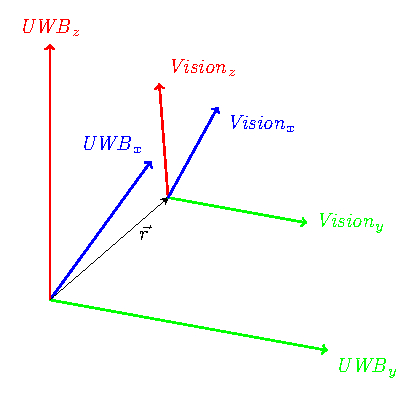
\includegraphics[width=0.5\textwidth]{figures/coordination_system}
	\caption{The two coordination systems relative to each other.}\label{fig:coordinationsystem}
\end{figure}

\subsection{ArUco}\label{subsec:aruco}
ArUco \cite{Aruco2014} presents itself as a minimal library for augmented reality applications based on OpenCV. ArUco is a marker system specialized for camera pose estimation in different applications such as augmented reality, robot localization, etc. ArUco contains an algorithm for the generation of markers as well as marker boards and an algorithm for the automatic detection of markers. A third contribution of ArUco is a solution to the occlusion problem in augmented reality applications which is not of interest for this semester project.

To get 3D vision coordinates, an ArUco marker was mounted on the object, as shown in \autoref{fig:target}, right in front of an \ac{UWB} target and an application was written which uses the ArUco library to read out the 3D coordinates of detected ArUco markers and saves them for later usage by the matching proceeder.
\begin{figure}[ht!]\centering
	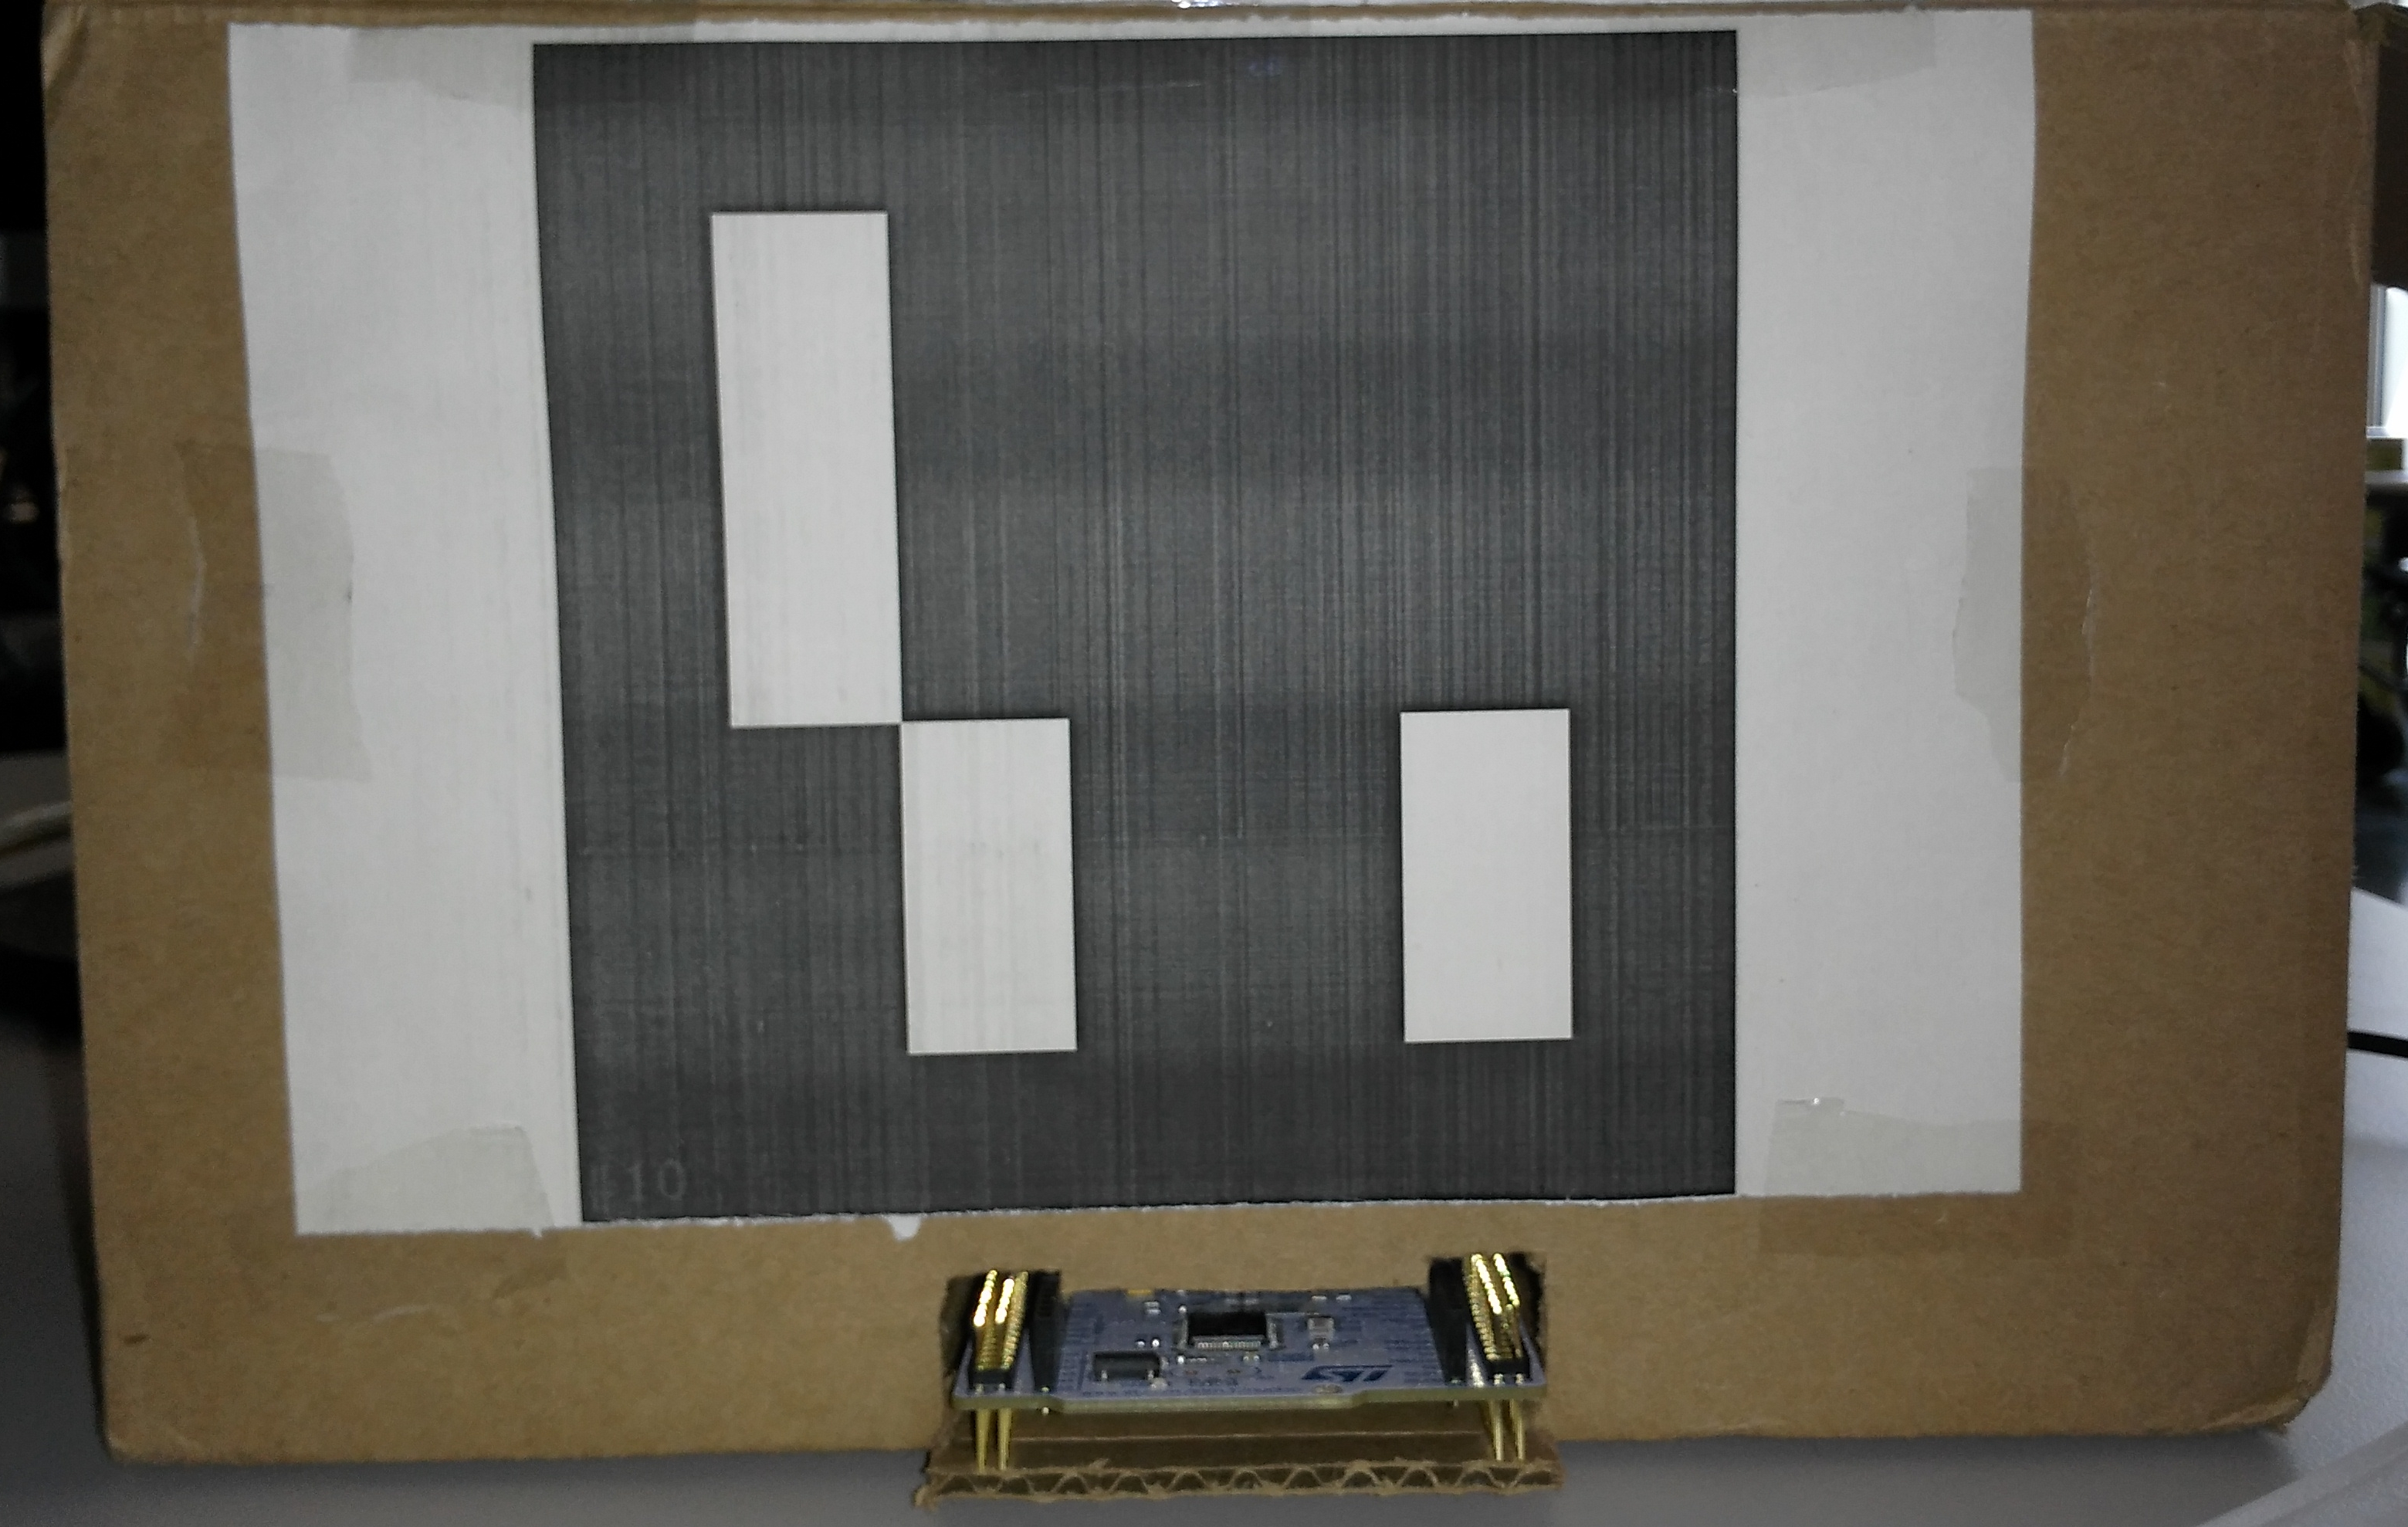
\includegraphics[width=0.5\textwidth]{figures/Box_cut.jpg}
	\caption{ArUco marker and \ac{UWB} target.}\label{fig:target}
\end{figure}

\subsection{Kabsch}
The Kabsch algorithm \cite{Kabsch:a12999} calculates the optimal rotation matrix and translation vector that minimizes the root mean squared deviation between two sets of corresponding points. In this semester project, the Kabsch algorithm determines the optimal rotation matrix and translation vector between the coordination systems of the \ac{UWB} system an the one of the camera.

\subsection{Matching proceeder}\label{subsec:matching}
For the matching proceeder, a Matlab script was written, shown in \autoref{lst:matching}, which calculates the mean of the \ac{UWB} and the vision (ArUco) coordinates, centralizes the coordinates of both, calculates the scale from the centralized coordinates, scales the vision (ArUco) coordinates and finally executes the Kabsch algorithm to calculate the rotation matrix $\textbf{U}$, the translation $\vec r$ and the least root mean squared error $\text{lrms}$.

To transform 3D points from the \ac{UWB} coordinate system to the vision coordinate system the translation $\vec r$ is applied to the 3D coordinate and the then rotation matrix $\textbf{U}$ and the scale is applied as shown in \autoref{eq:transformation}

\begin{equation}\label{eq:transformation}
	\begin{bmatrix}
		x_{\textit{Vision}} \\
		y_{\textit{Vision}} \\
		z_{\textit{Vision}}
	\end{bmatrix} = \frac{1}{\mathit{scale}} \cdot \textbf{U}
	\Bigg( \begin{bmatrix}
		x_{\textit{UWB}} \\
		y_{\textit{UWB}} \\
		z_{\textit{UWB}}
	\end{bmatrix} - \vec r \Bigg)
\end{equation}

To transform the covariance matrix $\textbf{C}$ from the \ac{UWB} coordinate system to the vision coordinate system, a new rotation matrix $\textbf{U}' \in \mathbb{R}^{6x6}$ has to be applied to the covariance matrix in the \ac{UWB} coordinate system like

\begin{equation}
	\textbf{C}' = \frac{1}{\mathit{scale}^2} \textbf{U}' \textbf{C} \textbf{U}'^T
\end{equation}
where
\begin{equation}
	\textbf{U}' =
	\begin{bmatrix}
		\textbf{U} & \textbf{0} \\
		\textbf{0} & \textbf{U}
	\end{bmatrix}
\end{equation}

The determined rotation matrix $\textbf{U}$ and the translation vector $\vec r$ applied on a set of measured points by the \ac{UWB} systems together with the set of measured points by ArUco results in a data set as shown in \autoref{fig:matching}

\lstset{language=Matlab}
\begin{lstlisting}[frame=single, caption=Matching proceeder, label=lst:matching]
% Calculate mean
mean_uwb = mean(uwb(1:3,:), 2);
mean_aruco = mean(aruco(1:3,:), 2);
	
% normalize data	
aruco_centred(1,:) = (aruco(1,:) - ...
		mean_aruco(1)*ones(1,length(aruco(1,:))));
aruco_centred(2,:) = (aruco(2,:) - ...
		mean_aruco(2)*ones(1,length(aruco(1,:))));
aruco_centred(3,:) = (aruco(3,:) - ...
		mean_aruco(3)*ones(1,length(aruco(1,:))));

uwb_centred(1,:) = uwb(1,:) - ...
		mean_uwb(1)*ones(1,length(uwb(1,:)));
uwb_centred(2,:) = uwb(2,:) - ...
		mean_uwb(2)*ones(1,length(uwb(2,:)));
uwb_centred(3,:) = uwb(3,:) - ...
		mean_uwb(3)*ones(1,length(uwb(3,:)));
	
% calculate scale
scale = norm(uwb_centred)/norm(aruco_centred);
	
aruco = scale .* aruco;
	
	
[U, r, lrms] = Kabsch(aruco, uwb);
\end{lstlisting}



\begin{figure}[ht!]\centering
	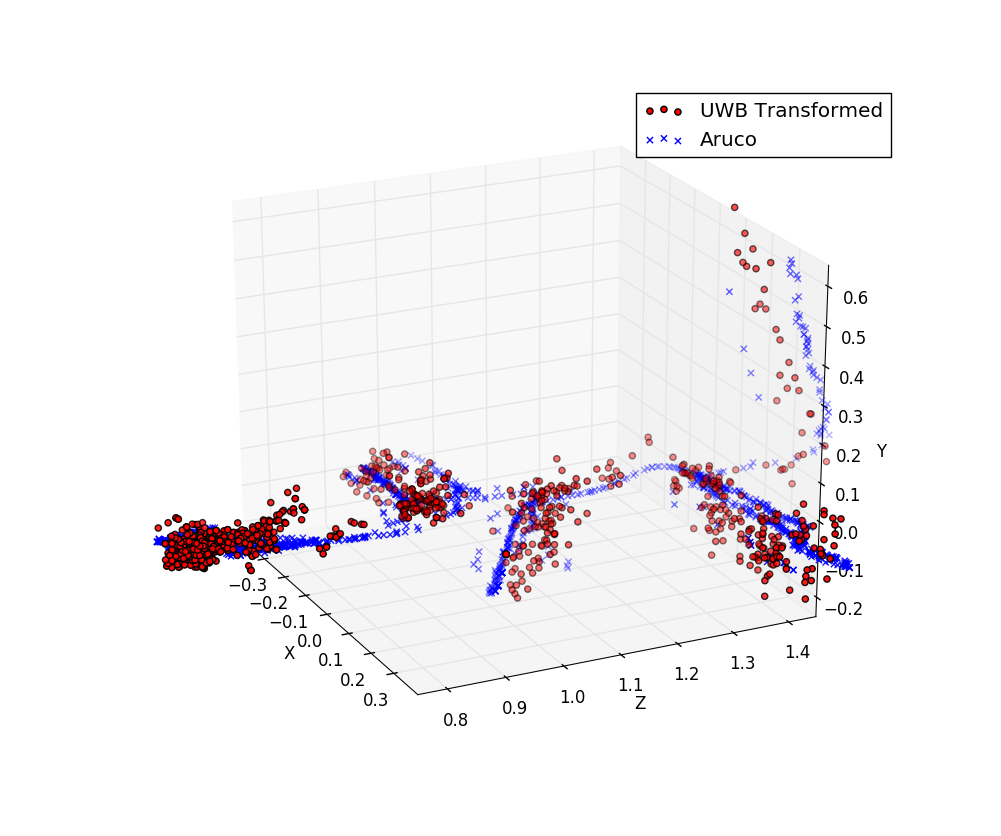
\includegraphics[width=1.0\textwidth]{figures/matching}
	\caption{Matching of the position set of ArUco and \ac{UWB}.}\label{fig:matching}
\end{figure} 

\section{\ac{ROS} setup}
In this semester project three different \ac{ROS} setups were used to perform the tasks of recording the video from the camera as well as recording the measurements from the \ac{UWB} system, collecting the data required for the matching proceeder and for the object tracking task.

The first setup to record the video and the measurement of the \ac{UWB} system is described in \autoref{subsec:recording}.

The setup to gain the required data to perform the matching proceeder explained in \autoref{subsec:matching}, is described in \autoref{subsec:kabsch}.

The third and last \ac{ROS} setup that was used in this semester project, is the setup introduced in \autoref{subsec:tracking}, which is used for the main task, of object tracking.

\subsection{Recording setup}\label{subsec:recording}
In the recording setup, shown in \autoref{fig:recording}, a rosbag node records the messages from the two nodes publish\_image and uwb. The message "/camera/video" from the publish\_image node is the image stream from the camera. The node uwb sends the message "/uwb/tracker" which consists of the position and the velocity of the target as well as their covariances.

\begin{figure}[h]\centering
	\includegraphics[width=0.8\textwidth]{figures/blockdiagram_recording}
	\caption{Block diagram of the \ac{ROS} nodes and messages for the recording setup.}\label{fig:recording}
\end{figure}

\subsection{Kabsch setup}\label{subsec:kabsch}
To save the required data to perform the matching proceeder described in \autoref{subsec:matching}, the setup, shown in \autoref{fig:kabsch}, was used. In this \ac{ROS} setup the node uwb\_aruco receives the messages "/camera/video" and "/uwb/tracker". It saves the positions measured by the \ac{UWB} system directly and performs the ArUco marker detection to get the positions detected by ArUco and also saves them.

\begin{figure}[h]\centering
	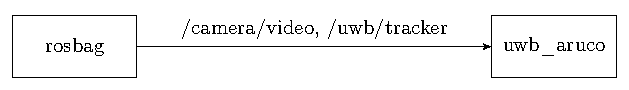
\includegraphics[width=0.8\textwidth]{figures/blockdiagram_kabsch}
	\caption{Block diagram of the \ac{ROS} nodes and messages for the Kabsch setup.}\label{fig:kabsch}
\end{figure}

\subsection{Tracking setup}\label{subsec:tracking}
This \ac{ROS} setup, shown in \autoref{fig:tracking}, is used for the main task, of tracking an object. In this setup, the node vision\_tracker performs the object tracking on the images it receives from the node rosbag in the messages "/camera/video". It then publishes the position of the tracked object in the messages "/vision\_tracker/vision\_coordinates". The node fusing receives the positions measured by the \ac{UWB} system in the messages "/uwb/tracker" as well as the positions of the object detected by the node vision\_tracker in the messages "/vision\_tracker/vision\_coordinates. With an Extended Kalman Filter (EKF), described in \autoref{ch:fusing}, the node fusing estimates the position of the tracked object.

\begin{figure}[h]\centering
	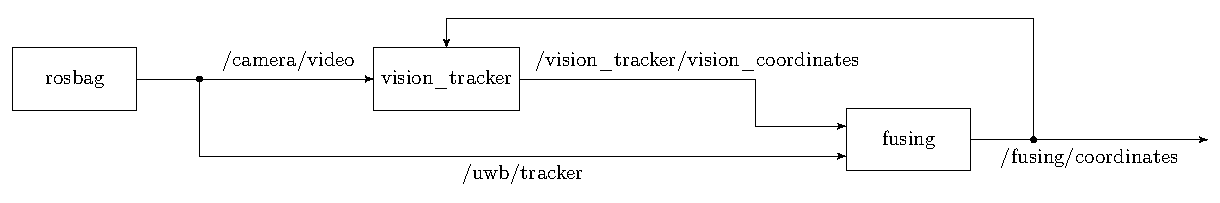
\includegraphics[width=1.0\textwidth]{figures/blockdiagram_tracking}
	\caption{Block diagram of the \ac{ROS} nodes and messages for the tracking setup.}\label{fig:tracking}
\end{figure}

\chapter{Fusing of the two measurement sources}\label{ch:fusing}

The position of the object is estimated with an Extended Kalman Filter (EKF), using a model of the system and the measurements from the UWB as well as from the vision tracker. A block diagram of this pipeline is shown in \autoref{fig:block}.

\begin{figure}[h]\centering
	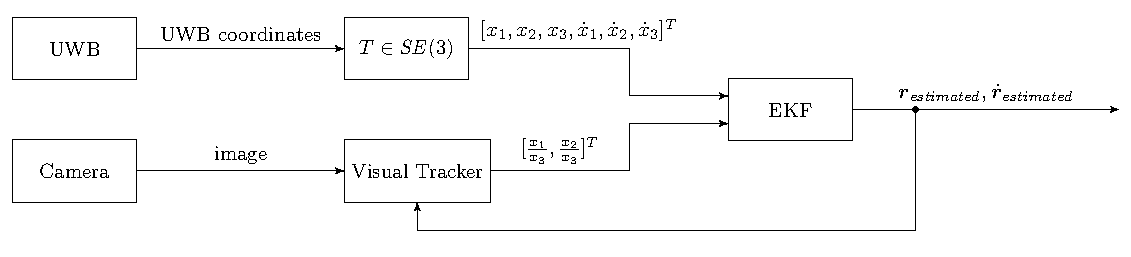
\includegraphics[width=1.0\textwidth]{figures/blockdiagram_setup}
	\caption{Block diagram of the EKF pipeline.}\label{fig:block}
\end{figure}

\section{Extended Kalman Filter (EKF)}

\subsection{System Model}
The state $\vec x = [\vec r, \dot{\vec{r}}]^T$ of our model consists of a position $\vec r \in \mathbb{R}^3$ and a velocity $\dot{\vec r} \in \mathbb{R}^3$.
The discrete process model with timestep $\Delta T$ is given by
\begin{equation}
	\vec x(k) = \vec q_{k-1}(\vec x(k-1), \vec v(k-1))
\end{equation}
with
\begin{equation}
  q_{k-1}(\vec x(k-1), \vec v(k-1)) = \textbf{B} \vec x(k-1) + \vec v(k-1)
\end{equation}
where 
\begin{align}
	\textbf{B} =
	\begin{pmatrix}
		\textbf{I}_3 & \Delta \textbf{T}\\
		\textbf{0} & \textbf{I}_3
	\end{pmatrix}
\end{align} 

and
\begin{equation}
	\vec v(k-1) \sim \mathcal{N}(\vec 0, \textbf{Q})
\end{equation}
where
\begin{align}
	\textbf{Q} =
	\begin{pmatrix}
		\textbf{I}_3 & \textbf{0}\\
		\textbf{0} & \textbf{q}_v
	\end{pmatrix}
\end{align}
and $\textbf{q}_v \in \mathbb{R}^{3\times3}$ is the velocity covariance of the process noise.

There are two possible measurements. The first measurement is a direct measurement of the state $\vec x$ from ultra-wideband (UWB) multilateration:
\begin{equation}
	\vec z_1(k) = \vec h_{k,1}(\vec x(k), \vec w_1(k))
\end{equation}
with
\begin{equation}
  \vec h_{k,1}(x(k), w_1(k)) = \textbf{H}_1 \vec x(k) + \vec w_1(k)
\end{equation}
where
$$\textbf{H}_1 = \textbf{I}_6$$
and
$$\vec \omega_1(k) \sim \mathcal{N}(\vec 0, \textbf{R}_1)$$
where $\textbf{R}_1 \in \mathbb{R}^{6\times6}$ is the covariance of the UWB measurement.
The second measurement is a projection of the position $\vec r$ as seen by a camera:
\begin{equation}
	\vec z_2(k) = \vec h_{k,2}(\vec x(k), \vec w_2(k))
\end{equation}
with
\begin{equation}
  \vec h_{k,2}(\vec x(k), \vec w_2(k)) = \textbf{H}_2(\vec x(k)) + \vec w_2(k)
\end{equation}
where
\begin{equation}
	\textbf{H}_2(\vec x) = [\frac{x_1}{x_3}, \frac{x_2}{x_3}]^T \in \mathbb{R}^2\\
\end{equation}
and
\begin{equation}
  \vec \omega_2(k) \sim \mathcal{N}(\vec 0, \textbf{R}_2)
\end{equation}

where $\textbf{R}_2 \in \mathbb{R}^{2\times2}$ is the covariance of the camera measurement.

\subsection{The Extended Kalman Filter steps}
There are two steps which have to be performed in an iterative fashion when running the Extended Kalman Filter (EKF).

\subsubsection{Step 1: Prior update/Prediction step}
In the first step, a prediction for the mean of the states $\hat{\vec x}_p(k)$ and the co-variance matrix $\textbf{P}_p(k)$ is calculated from the linearized system model.
\begin{align}
  \hat{\vec x}_p(k) &=  q_{k-1}(\hat{\vec x}_m(k-1), 0) = \textbf{B} \hat{\vec x}_m(k-1)\\
	\textbf{P}_p(k) &= {\textbf{A}}(k-1) \textbf{P}_m(k-1) {\textbf{A}}^T(k-1) + \textbf{L}(k-1) \textbf{Q} \textbf{L}^T(k-1) \label{eq:ekf_s1}
\end{align}
where
\begin{align}
  \textbf{A}(k-1) & = \frac{\partial q_{k-1}(\hat{\vec x}_m(k-1), 0)}{\partial \vec x}\\
  & =  \frac{\partial}{\partial \vec x} \big(\textbf{B} \vec x(k-1) + \vec v(k-1)\big)\\
	& = \textbf{B}(k-1)\\
  \textbf{L}(k-1) & = \frac{\partial q_{k-1}(\hat{\vec x}_m(k-1), 0)}{\partial \vec v}\\
  & = \frac{\partial}{\partial \vec v} \big( \textbf{B} \vec x(k-1) + \vec v(k-1)\big)\\
	& = \textbf{I}_6
\end{align}
and with the initial values $\hat{\vec x}_m(0) = x_0$ and $\textbf{P}_m(0) = \textbf{0}$.
Therefore equation \ref{eq:ekf_s1} becomes
$$\textbf{P}_p(k) = \textbf{B}(k-1)\textbf{P}_m(k-1)\textbf{B}^{T}(k-1) + \textbf{Q}$$

\subsubsection{Step 2: A posteriori update/Measurement update step}
In the second step, the information gained from the measurements are used to perform an a posteriori update, resulting in a updated mean of the states $\hat{\vec x}_m(k)$ and an updated co-variance matrix $\textbf{P}_m(k)$.
\begin{align}
	\textbf{K}(k) = \textbf{P}_p(k) \textbf{H}^T(k) \Big( \textbf{H}(k) \textbf{P}_p(k) \textbf{H}^T(k) + \textbf{M}(k) \textbf{R}(k) \textbf{M}^T(k)\Big)^{-1} \label{eq:ekf_s2}\\
	\hat{\vec x}_m(k) = \hat{\vec x}_p(k) + \textbf{K}(k) \Big( \vec z(k) - \begin{bmatrix}
	\vec h_{k,1}(\hat{\vec x}_p(k), 0)\\
	\vec h_{k,2}(\hat{\vec x}_p(k), 0))
	\end{bmatrix} \Big)\\
	\textbf{P}_m(k) = \big( \textbf{I} - \textbf{K}(k)\textbf{H}(k)\big) \textbf{P}_p(k)
\end{align}
where
\begin{align}
  \textbf{H}(k) &= \begin{bmatrix}
    \frac{\partial h_k(\hat{\vec x}_p(k), 0)}{\partial \vec x}
  \end{bmatrix}\\
  &= \begin{bmatrix}
		\frac{\partial}{\partial \vec x} \big( \textbf{H}_1 \hat{\vec x}(k) + \vec \omega_1(k) \big)\\
		\frac{\partial}{\partial \vec x} \big( \textbf{H}_2(\hat{\vec x}(k)) + \vec \omega_2(k) \big)
	\end{bmatrix}\\
	&= \begin{bmatrix}
		\textbf{I}_6\\
		\frac{1}{\hat{x}_3} & 0 & -\frac{\hat{x}_1}{\hat{x}^2_3} & 0 & 0 & 0\\
		0 & \frac{1}{\hat{x}_3} & -\frac{\hat{x}_2}{\hat{x}^2_3} & 0 & 0 & 0
	\end{bmatrix}\\
  \textbf{M}(k) & = \begin{bmatrix}
    \frac{\partial h_k(\hat{\vec x}_p(k), 0)}{\partial \vec w}
  \end{bmatrix}\\
  &= \begin{bmatrix}
		\frac{\partial}{\partial \vec \omega} \big( \textbf{H}_1 \hat{\vec x}(k) + \vec \omega_1(k) \big)\\
		\frac{\partial}{\partial \vec \omega} \big( \textbf{H}_2(\hat{\vec x}(k)) + \vec \omega_2(k) \big)
	\end{bmatrix}\\
	&= \textbf{I}_8
\end{align}
Therefore equation \ref{eq:ekf_s2} becomes
$$\textbf{K}(k) = \textbf{P}_p(k) \textbf{H}^T(k) \Big( \textbf{H}(k) \textbf{P}_p(k) \textbf{H}^T(k) + \begin{bmatrix}
	\textbf{R}_1 & \textbf{0}\\
	\textbf{0} &\textbf{R}_2
\end{bmatrix} \Big)^{-1}$$

\subsection{Implementation}
The implementation of the EKF was done in a Python script within the ROS environment. For more details please see \cite{Ziegler:2016}.

\begin{figure}[ht!]\centering
	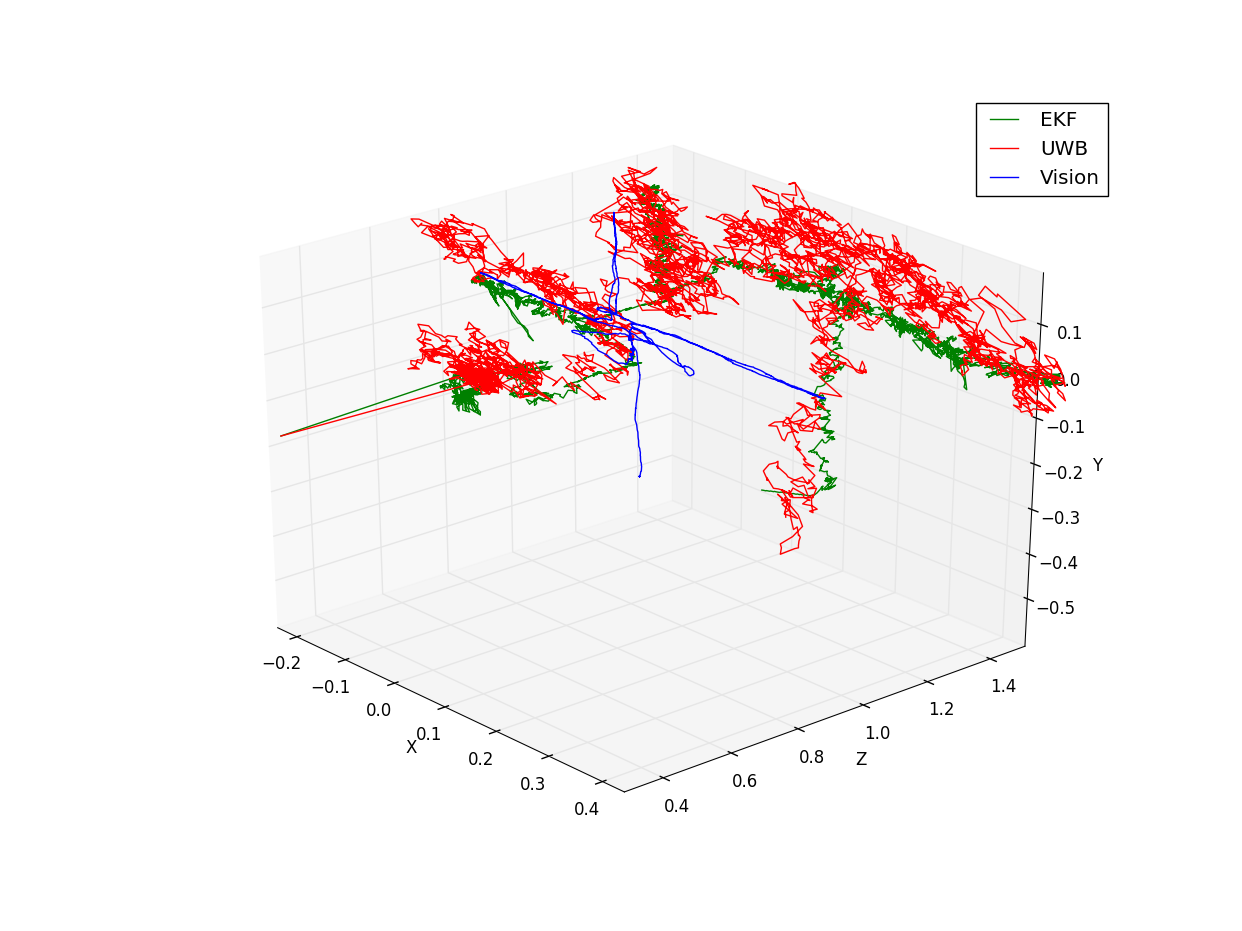
\includegraphics[width=1.0\textwidth]{figures/state_track}
	\caption{3D pot of the measured point by the UWB (red), the measured point by the vision tracker (blue) and the fused positions (green)}\label{fig:statetrack}
\end{figure}

\chapter{Experiment and Results}

\section{Experiment}
To measure the accuracy of the developed system, the ROS setup similar as described in \autoref{subsec:tracking} was used. The EKF works in the camera coordinate systems with approximately $80\mathit{Hz}$. To eases the whole handling, the experiments were recorded with rosbag and then afterwards off-line evaluated with a separate python script.

To have a ground truth to compare with, the 3D coordinates of the tracked object measured by a motion capture system (VICON) were additionally recorded.

For the comparison between the accuracy of the UWB system and the one of the EKF, both systems were compared with the mentioned ground truth by the root mean squared error $$\textit{rmse} = \frac{1}{\#\text{ of elements}} \sum_i \sqrt{(x_{m,i} - x_{V,i})^2 + (y_{m,i} - y_{V,i})^2 + (z_{m,i} - z_{V,i})^2}$$
and by the root mean squared error of only the $x$ and $y$ axis
$$\textit{rmse}_{xy} = \frac{1}{\#\text{ of elements}} \sum_i \sqrt{(x_{m,i} - x_{V,i})^2 + (y_{m,i} - y_{V,i})^2}$$

where the subfix $m$ stands for measurement and represents coordinates which either come from the UWB system or from the EKF. The subfix $V$ on the other hand stands for VICON which is the ground truth in this experiment. 

\section{Results}
On several recorded experiments, the $\textit{rmse}$ and the $\textit{rmse}_{xy}$ of the EKF was significantly lower compared to the $\textit{rmse}$ and the $\textit{rmse}_{xy}$ of the UWB. The results of some experiments are listed in \autoref{tab:results}. A 3D plot of the measured coordinates by the VICON system (ground truth), the UWB system and the coordinates fused by the EKF from a data set is shown in \autoref{fig:evaluation}.

\begin{table}[ht!]
\begin{center}
\begin{tabular}{c|c|c|c|c}
	Experiment number & $\textit{rmse}$ of UWB & $\textit{rmse}$ of EKF & $\textit{rmse}_{xy}$ of UWB & $\textit{rmse}_{xy}$ of EKF\\ 
	\hline 
	1 & 0.0753 & 0.0278 & 0.0705 & 0.0171 \\
	2 & 0.0732 & 0.0290 & 0.0681 & 0.0169 \\ 
	%\hline 
\end{tabular}
\end{center}
\caption{Table with listed $\textit{rmse}$ and $\textit{rmse}_{xy}$ of the UWB system and the EKF for the different experiments.}
\label{tab:results}
\end{table}

\begin{figure}[ht!]\centering
	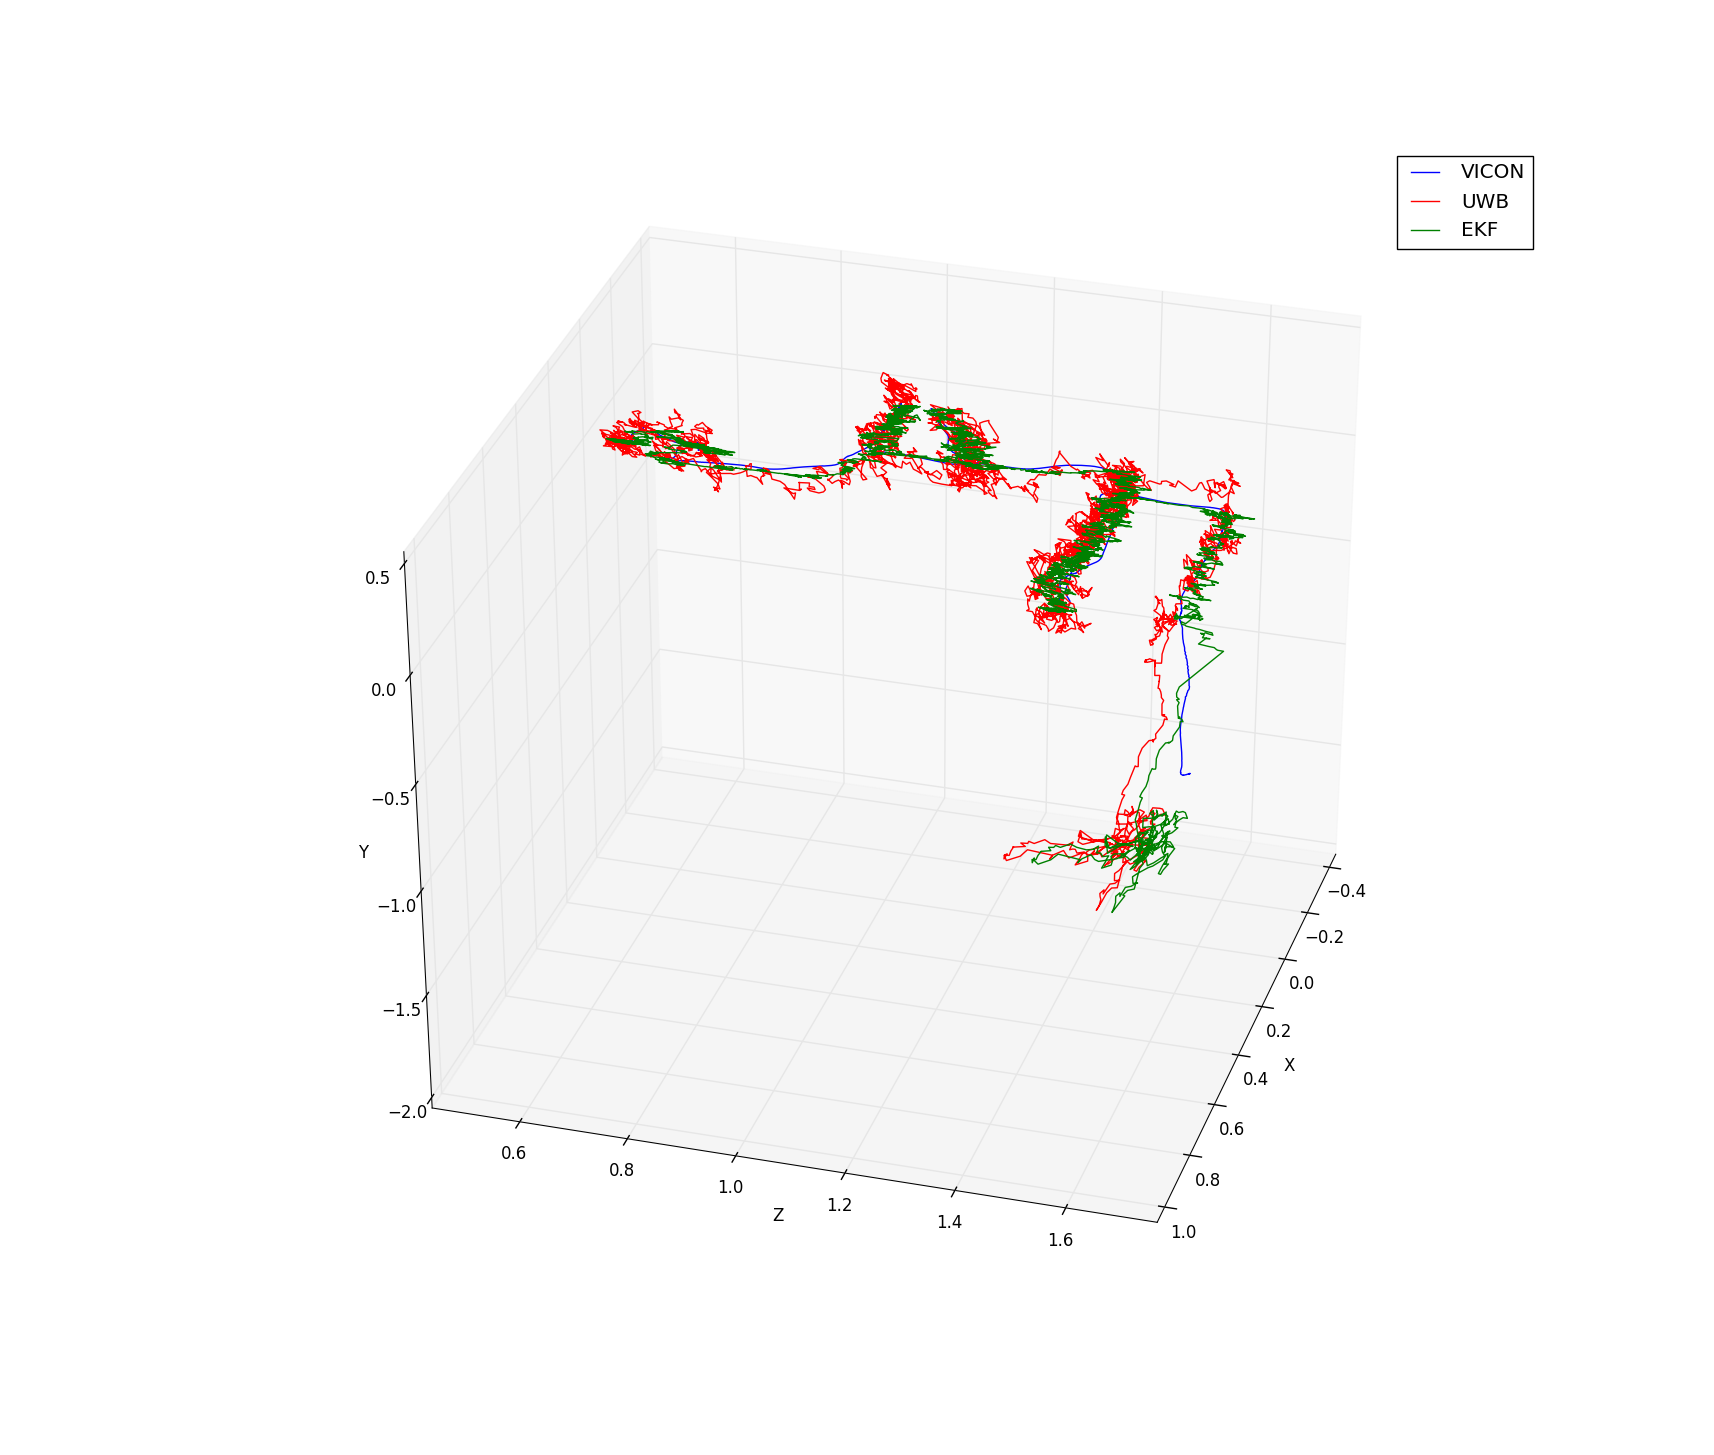
\includegraphics[width=1.0\textwidth]{figures/evaluation}
	\caption{3D pot of the measured coordinate points by the UWB system (red), the measured point by the VICON system (blue) and the fused positions (green)}\label{fig:evaluation}
\end{figure}

\chapter{Conclusion and Outlook}

\section{Conclusion}
The proposed method of fusing less accurate 3D coordinate measurements from the UWB system with more precise 2D pixel coordinate measurements from the vision based tracker with an Extended Kalman Filter has shown to improve the accuracy significantly compared to the coordinates measured solely by the UWB system. The idea of combining these two sources has therefore proven to be beneficial.

This semester project was meant to be a prove of concept and the proposed method could be applied in many applications in different fields as robotics, human-computer-interaction, entertainment, rescue, etc., to mention only a few.

\section{Outlook}
The UWB system used in this semester project runs with a frequency of approximately $80\mathit{Hz}$ as well as the implemented Extended Kalman Filter. If an UWB system with a higher frequency would be used, the currently in python implemented Extended Kalman Filter won't be able to process all the measurements provided by the UWB system and by the vision based tracker. To encounter this problem, a faster implementation in C++ would be conceivable.

The proposed fusing method does not contain any sophisticated re-detection system for the cases when the object goes out of the camera view. A re-detection based on the 3D coordinate measurements of the UWB system could improve the stability as well as the usability of the proposed method.\todo{(If redetection works somehow, adapt this part)}

So far the used UWB system has to be calibrated manually, for example with a motion capture system (VICON). With an ArUco marker and the ArUco library \cite{Aruco2014} an automated calibration proceeder for the UWB system could be developed which would simplify the setup of the whole system. 

Up to now, for the vision based tracker the desired object has to be marked manually by an user which restricts the usability of the system in many real-world applications. Automatic visual target detecting with the help of the information provided by the UWB system would widen the the application area of the proposed system.

In this semester project only one object at a time can be tracked. In many applications tracking of multiple targets is of interest. A multi target tracking system consisting of multiple objects equipped with distinguishable UWB targets and a vision based multi target tracker would allow to track multiple object simultaneously. 


% ---- END MAIN PART ----


\appendix
\clearpage
\renewcommand*{\chapterpagestyle}{myappendixpagestyle}

%% !TEX root = ../thesis.tex

\chapter{Information For The Few (Appendix)}

Nein, meine Texte les ich nicht, so nicht, st�hnte Oxmox. Er war mit Franklin, Rockwell und dem halbtaxgrauen Panther Weidemann in Memphis (Heartbreak Hotel) zugange. Sie warteten auf die fette Gill, um bei der Bank of Helvetica die Kapit�lchen in Kapital umzuwandeln. Oxmox liess nicht locker. Ich fleh euch an, rettet meine Copy, gebt meinem Body nochn Durchschuss! Kein Problem, erbarmte sich Old Face Baskerville, streichelte seinen Hund, zog seine einspaltige Poppl, legte an und traf! (Zeidank nichts Ernstes --- nurn bisschen Fraktur.) Oxmox: Danke, ist jetzt mit Abstand besser. Derweil jumpte der Fox leise over the Buhl, die sich mal wieder immerdar wie jedes Jahr gesellte. Diesmal war Guaredisch ihr Erw�hlter, weil seine Laufweite einem vollgetankten Bodoni entsprach und seine ungez�gelte Unterl�nge ihre Serifen so serafisch streifte, dass sie trotz Techtelmechtelei die magere Futura, jene zuverl�ssige und gern eingesetzte Langstreckenl�uferin, rechtsb�ndig �berholen konnten.

\section{Foo Bar Baz}

Nein, meine Texte les ich nicht, so nicht, st�hnte Oxmox. Er war mit Franklin, Rockwell und dem halbtaxgrauen Panther Weidemann in Memphis (Heartbreak Hotel) zugange. Sie warteten auf die fette Gill, um bei der Bank of Helvetica die Kapit�lchen in Kapital umzuwandeln. Oxmox liess nicht locker. Ich fleh euch an, rettet meine Copy, gebt meinem Body nochn Durchschuss! Kein Problem, erbarmte sich Old Face Baskerville, streichelte seinen Hund, zog seine einspaltige Poppl, legte an und traf! (Zeidank nichts Ernstes --- nurn bisschen Fraktur.) Oxmox: Danke, ist jetzt mit Abstand besser. Derweil jumpte der Fox leise over the Buhl, die sich mal wieder immerdar wie jedes Jahr gesellte. Diesmal war Guaredisch ihr Erw�hlter, weil seine Laufweite einem vollgetankten Bodoni entsprach und seine ungez�gelte Unterl�nge ihre Serifen so serafisch streifte, dass sie trotz Techtelmechtelei die magere Futura, jene zuverl�ssige und gern eingesetzte Langstreckenl�uferin, rechtsb�ndig �berholen konnten.

\section{Barontes}

Nein, meine Texte les ich nicht, so nicht, st�hnte Oxmox. Er war mit Franklin, Rockwell und dem halbtaxgrauen Panther Weidemann in Memphis (Heartbreak Hotel) zugange. Sie warteten auf die fette Gill, um bei der Bank of Helvetica die Kapit�lchen in Kapital umzuwandeln. Oxmox liess nicht locker. Ich fleh euch an, rettet meine Copy, gebt meinem Body nochn Durchschuss! Kein Problem, erbarmte sich Old Face Baskerville, streichelte seinen Hund, zog seine einspaltige Poppl, legte an und traf! (Zeidank nichts Ernstes --- nurn bisschen Fraktur.) Oxmox: Danke, ist jetzt mit Abstand besser. Derweil jumpte der Fox leise over the Buhl, die sich mal wieder immerdar wie jedes Jahr gesellte. Diesmal war Guaredisch ihr Erw�hlter, weil seine Laufweite einem vollgetankten Bodoni entsprach und seine ungez�gelte Unterl�nge ihre Serifen so serafisch streifte, dass sie trotz Techtelmechtelei die magere Futura, jene zuverl�ssige und gern eingesetzte Langstreckenl�uferin, rechtsb�ndig �berholen konnten.


\section{A Long Table with Booktabs}


{\scriptsize
\begin{longtable}{clccccccc}
\caption[Wordlist]{A sample list of words.}\\
\toprule
ID & Word & Word Length & WD & ETL & PTL &  WDplus \\
\midrule
\endfirsthead
\caption[]{(Continued)}\\
\toprule
ID & Word & Word Length & WD & ETL & PTL &  WDplus \\
\midrule
\endhead
\midrule
\multicolumn{9}{c}{continued on next page}\\
\bottomrule
\endfoot
%\bottomrule
\endlastfoot
\hline
1 & Eis & 3 & 4 & 0.42 & 1.83 & 0.19 \\ \hline
2 & Mai & 3 & 5 & 0.49 & 1.92 & 0.19 \\ \hline
3 & Art & 3 & 5 & 0.27 & 1.67 & 0.14 \\ \hline
4 & Uhr & 3 & 5 & 0.57 & 1.87 & 0.36 \\ \hline
5 & Rat & 3 & 5 & 0.36 & 1.71 & 0.14 \\ \hline
6 & weit & 4 & 6 & 0.21 & 1.65 & 0.25 \\ \hline
7 & eins & 4 & 6 & 0.38 & 1.79 & 0.26 \\ \hline
8 & Wort & 4 & 6 & 0.30 & 1.62 & 0.20 \\ \hline
9 & Wolf & 4 & 6 & 0.18 & 1.54 & 0.19 \\ \hline
10 & Wald & 4 & 6 & 0.31 & 1.63 & 0.19 \\ \hline
11 & Amt & 3 & 6 & 0.30 & 1.67 & 0.14 \\ \hline
12 & Wahl & 4 & 7 & 0.36 & 1.77 & 0.42 \\ \hline
13 & Volk & 4 & 7 & 0.45 & 1.81 & 0.20 \\ \hline
14 & Ziel & 4 & 7 & 0.48 & 1.78 & 0.42 \\ \hline
15 & vier & 4 & 7 & 0.38 & 1.81 & 0.42 \\ \hline
16 & Kreis & 5 & 7 & 0.26 & 1.62 & 0.33 \\ \hline
17 & Preis & 5 & 7 & 0.28 & 1.51 & 0.33 \\ \hline
18 & Re-de & 4 & 7 & 0.22 & 1.56 & 0.33 \\ \hline
19 & Saal & 4 & 7 & 0.75 & 2.10 & 0.43 \\ \hline
20 & voll & 4 & 7 & 0.48 & 1.82 & 0.24 \\ \hline
21 & weiss & 5 & 7 & 0.21 & 1.59 & 0.36 \\ \hline
22 & �r-ger & 5 & 7 & 1.16 & 2.69 & 0.59 \\ \hline
23 & bald & 4 & 7 & 0.18 & 1.56 & 0.19 \\ \hline
24 & hier & 4 & 7 & 0.40 & 1.70 & 0.43 \\ \hline
25 & neun & 4 & 7 & 0.17 & 1.52 & 0.26 \\ \hline
26 & sehr & 4 & 7 & 0.36 & 1.85 & 0.43 \\ \hline
27 & Jahr & 4 & 7 & 0.50 & 1.82 & 0.43 \\ \hline
28 & Gold & 4 & 7 & 0.04 & 1.35 & 0.20 \\ \hline
29 & T�-ter & 5 & 8 & 0.15 & 1.39 & 0.59 \\ \hline
30 & Tei-le & 5 & 8 & 0.30 & 1.71 & 0.46 \\ \hline
31 & Na-tur & 5 & 8 & 0.18 & 1.59 & 0.41 \\ \hline
32 & Feu-er & 5 & 8 & 0.30 & 1.71 & 0.45 \\ \hline
33 & Rol-le & 5 & 8 & 0.15 & 1.46 & 0.45 \\ \hline
34 & Rock & 4 & 8 & 0.29 & 1.68 & 0.25 \\ \hline
35 & Spass & 5 & 8 & 0.28 & 1.64 & 0.32 \\ \hline
36 & G�s-te & 5 & 8 & 0.49 & 1.75 & 0.66 \\ \hline
37 & En-de & 4 & 8 & 0.36 & 1.72 & 0.33 \\ \hline
38 & Kunst & 5 & 8 & 0.26 & 1.59 & 0.35 \\ \hline
39 & Li-nie & 5 & 8 & 0.45 & 1.88 & 0.63 \\ \hline
40 & B�u-me & 5 & 8 & 0.48 & 1.92 & 0.45 \\ \hline
41 & B�h-ne & 5 & 9 & 0.94 & 2.48 & 0.62 \\ \hline
42 & Bahn & 4 & 9 & 0.21 & 1.62 & 0.42 \\ \hline
43 & B�r-ger & 6 & 9 & 0.38 & 1.70 & 0.65 \\ \hline
44 & Druck & 5 & 9 & 0.60 & 2.03 & 0.31 \\ \hline
45 & zehn & 4 & 9 & 0.41 & 1.84 & 0.42 \\ \hline
46 & Va-ter & 5 & 9 & 0.36 & 1.78 & 0.40 \\ \hline
47 & Angst & 5 & 9 & 0.29 & 1.56 & 0.35 \\ \hline
48 & lei-der & 6 & 9 & 0.13 & 1.47 & 0.52 \\ \hline
49 & h�u-fig & 6 & 9 & 0.82 & 2.31 & 0.52 \\ \hline
50 & le-ben & 5 & 9 & 0.38 & 1.85 & 0.40 \\ \hline
51 & aus-ser & 6 & 9 & 1.20 & 2.26 & 0.57 \\ \hline
52 & be-vor & 5 & 9 & 1.28 & 2.75 & 0.39 \\ \hline
53 & Kai-ser & 6 & 9 & 0.92 & 2.37 & 0.53 \\ \hline
54 & Markt & 5 & 9 & 0.23 & 1.58 & 0.28 \\ \hline
55 & Os-ten & 5 & 9 & 0.21 & 1.54 & 0.48 \\ \hline
56 & Krieg & 5 & 9 & 0.33 & 1.67 & 0.50 \\ \hline
57 & Mann & 4 & 9 & 0.31 & 1.47 & 0.25 \\ \hline
58 & Hal-le & 5 & 9 & 0.24 & 1.65 & 0.45 \\ \hline
59 & heu-te & 5 & 9 & 0.44 & 1.87 & 0.46 \\ \hline
60 & in-nen & 5 & 10 & 0.36 & 1.80 & 0.45 \\ \hline
61 & Na-men & 5 & 10 & 0.28 & 1.72 & 0.41 \\ \hline
62 & jetzt & 5 & 10 & 0.70 & 2.07 & 0.32 \\ \hline
63 & kei-ner & 6 & 10 & 0.28 & 1.62 & 0.53 \\ \hline
64 & Schu-le & 6 & 10 & 1.02 & 2.12 & 0.48 \\ \hline
65 & Ar-beit & 6 & 10 & 0.34 & 1.70 & 0.52 \\ \hline
66 & An-teil & 6 & 10 & 0.27 & 1.63 & 0.53 \\ \hline
67 & di-rekt & 6 & 10 & 0.67 & 2.04 & 0.47 \\ \hline
68 & vor-her & 6 & 10 & 0.78 & 2.25 & 0.47 \\ \hline
69 & wol-len & 6 & 10 & 0.44 & 1.85 & 0.51 \\ \hline
70 & Kampf & 5 & 10 & 0.70 & 1.96 & 0.27 \\ \hline
71 & �n-dern & 6 & 10 & 1.18 & 2.62 & 0.65 \\ \hline
72 & lau-fen & 6 & 10 & 0.21 & 1.64 & 0.52 \\ \hline
73 & Eu-ro-pa & 6 & 10 & 0.23 & 1.53 & 0.66 \\ \hline
74 & statt & 5 & 10 & 1.61 & 2.86 & 0.39 \\ \hline
75 & Wes-ten & 6 & 10 & 0.29 & 1.60 & 0.54 \\
\bottomrule
\label{tab:wordlist}
\end{longtable}
}

\clearpage
\renewcommand*{\chapterpagestyle}{empty}

%\nocite{*}
\cleardoublepage
\phantomsection
\addcontentsline{toc}{chapter}{Bibliography}
\bibliography{graphics}

\end{document}
